\chapter{ Resultados Experimentais }
\label{cap:resultados}
\section{Experimentos}




\subsection{Abordagem Não-Temporal}

Para esses modelos como Redes Neurais, Árvores de Decisão e Regressões
Lineares, separamos os dados em treino e validação, normalizamos as variáveis e
treinamos os modelos. 

\subsubsection{Divisão dos dados entre treino e validação}

Para que obtenhamos um modelo que generalize em um novo conjunto de dados
inéditos, devemos usar parte dos dados que possuímos não para treinar o modelo,
mas para testá-lo. O erro nesse conjunto de dados separados apenas para teste é
chamado de erro de validação, e o usamos como uma estimativa da capacidade de
generalização dos modelos de aprendizagem automática.

\begin{figure}[H]
  \centering
  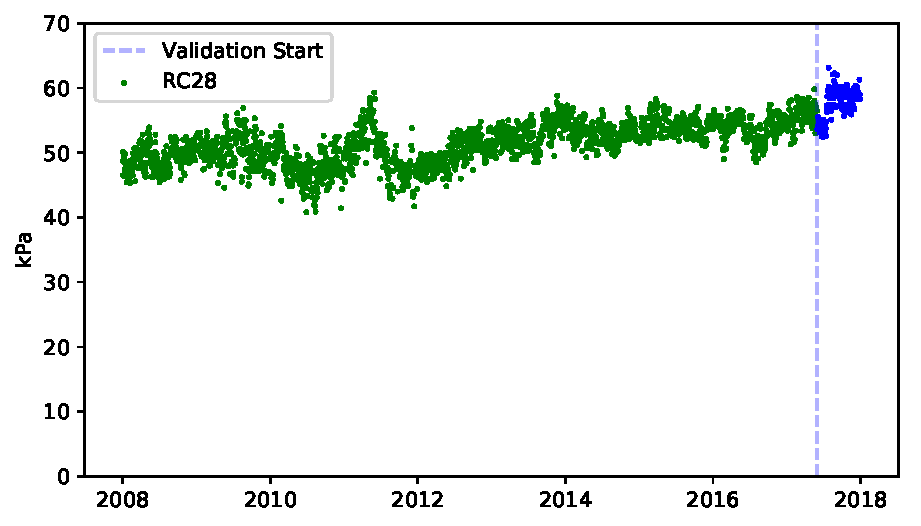
\includegraphics[width=0.9\columnwidth]{train_dev.pdf}
  \caption{Divisão do dataset para a saída RC28, os pontos verdes foram usados para
    treino e os pontos azuis usados para validação.}
  \label{fig:divrc28}
\end{figure}

Foram usadas implementacões dos modelos fornecidos pela biblioteca Sklearn.
As avaliações de RMSE de todo o conjunto de validação estão apresentados por modelos na Imagem~\ref{fig:linmodels}  

\begin{figure}[H]
  \centering
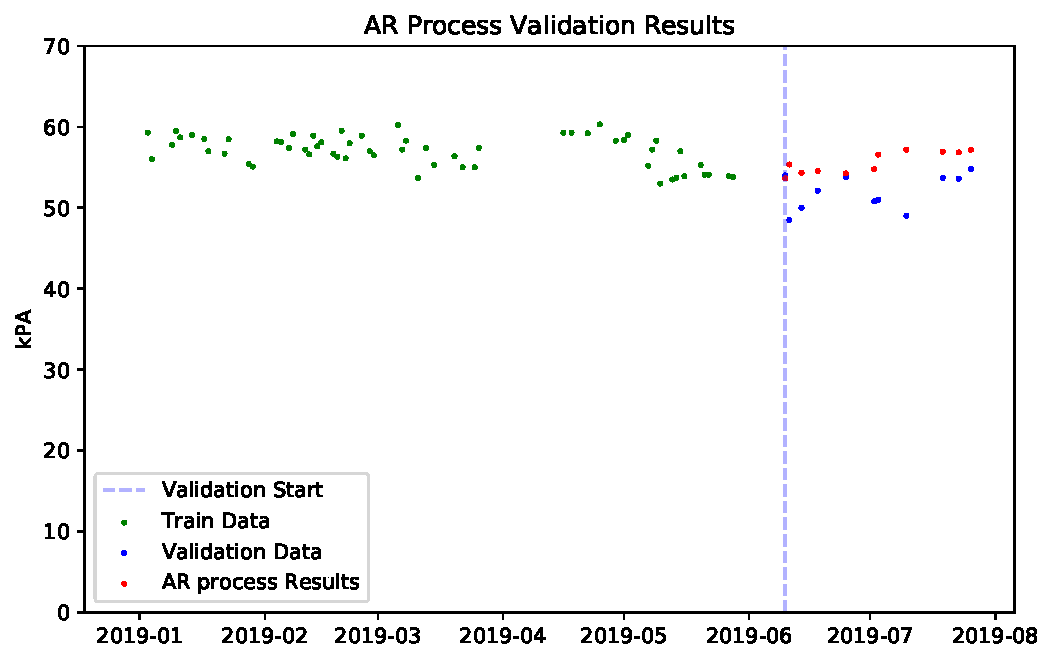
\includegraphics[width=0.9\columnwidth]{linear_exp.pdf}
\caption{Predições nos dados de validação nos experimentos com modelos não-temporais. }
\label{fig:linmodels}
\end{figure}

Na Tabela~\ref{tb:rmse_lin} reportamos os erros para predições imediatamente
após o fim do último dia de dados usados para treino. Iremos mostrar o
erro para o dia seguinte, três dias depois e então uma semana após o último dia
de dados usados para treinamento.

\begin{center}
\begin{table}[htbp]
\caption{RMSE values by forecast span}
\centering
\begin{tabular}{rr}
\hline
 Regressão Linear & RMSE\\
\hline
24h & 2.94\\
3d & 0.13\\
7d & 5.43\\
\hline
Rede Neural & RMSE\\
\hline
24h & 3.70\\
3d & 1.26\\
7d & 6.04\\
\hline
Random Forest & RMSE\\
\hline
24h & 1.61\\
3d & 1.36\\
7d & 5.83\\
\end{tabular}

\label{tb:rmse_lin}
\end{table}
\end{center}

 Reportamos distribuição dos valores previstos, até 1 mês após a data
onde começam os dados de validação (i.e. os dados não usamos para treinamento), a Imagem \ref{fig:distr_lin} permite comparar as distribuições previstas pelos 3 modelos:

\begin{figure}[H]
\label{fig:distr_lin}
\centering
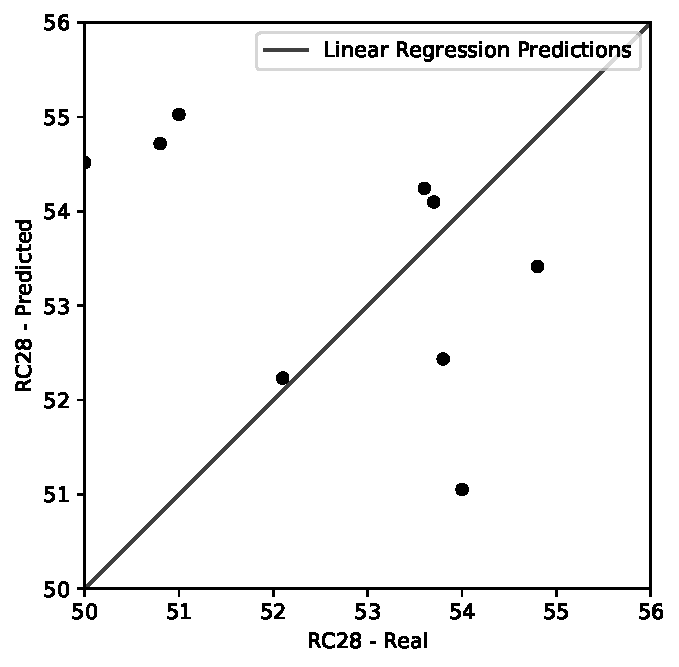
\includegraphics[width=.3\textwidth]{qq-LinearRegression.pdf} \hfill
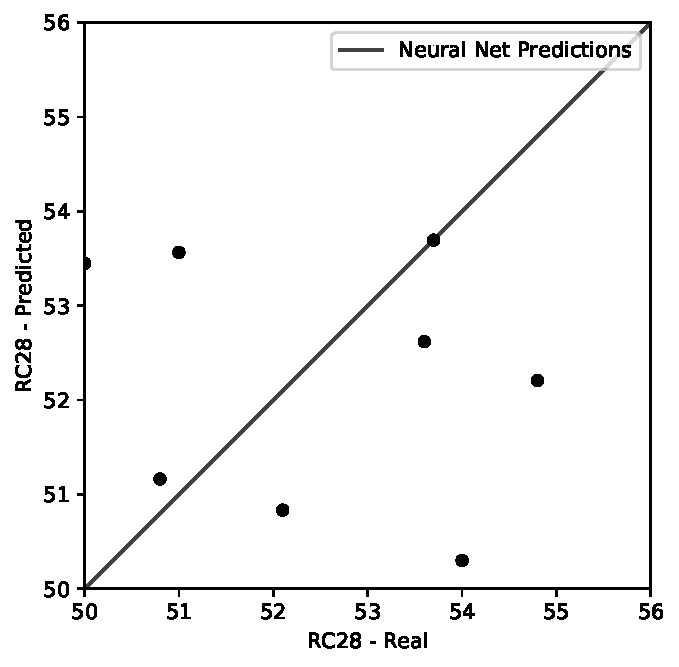
\includegraphics[width=.3\textwidth]{qq-NeuralNet.pdf} \hfill
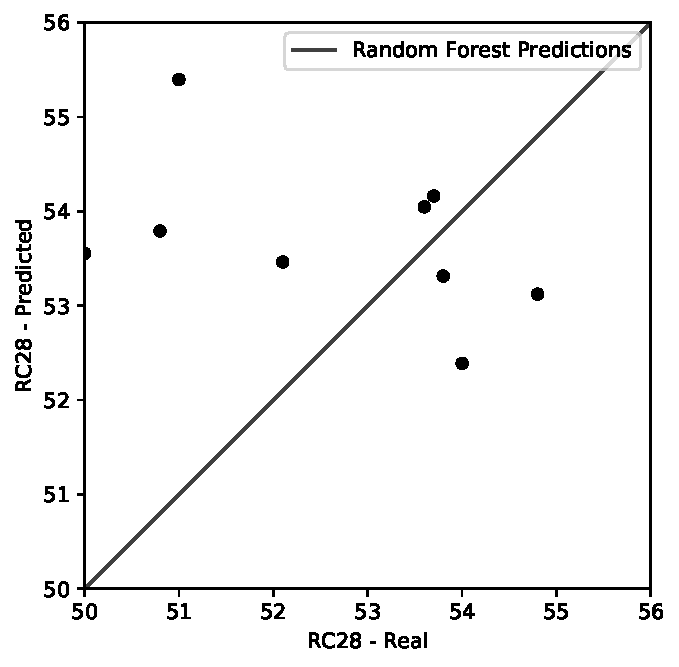
\includegraphics[width=.3\textwidth]{qq-RandomForest.pdf} 
\caption{Valores reais plotados contra os valores previstos para análise da distribuição aprendida por cada modelo} 
\end{figure}

Para modelagem de séries temporais, é comum se estudar o resíduo das
predições. É assumido em uma tarefa de regressão que o resíduo é distribuído
normalmente e com média zero.

\begin{figure}[H]
  \label{fig:res_lin}
  \centering
  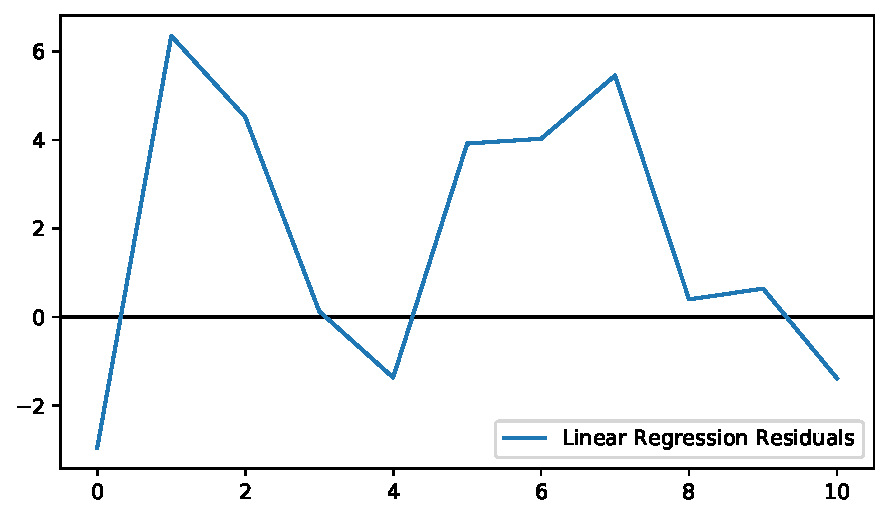
\includegraphics[width=.3\textwidth]{residuals-LinearRegression.pdf} \hfill
  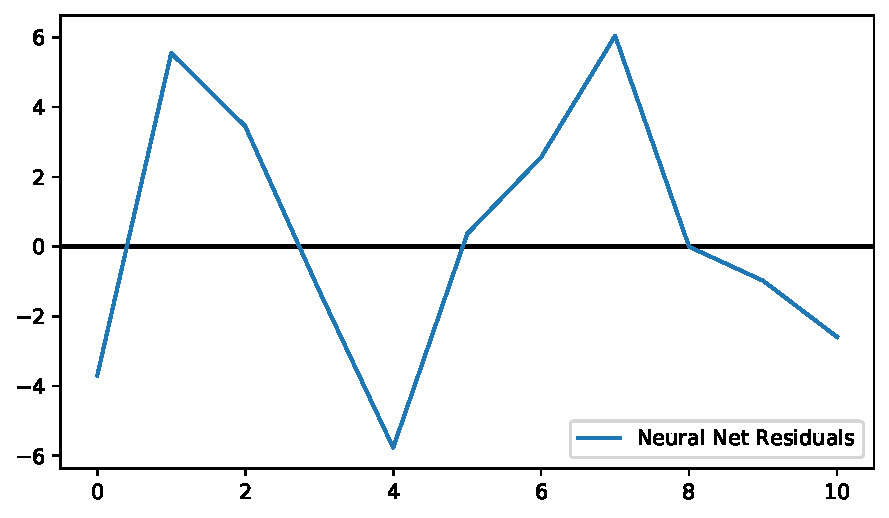
\includegraphics[width=.3\textwidth]{residuals-NeuralNet.pdf} \hfill
  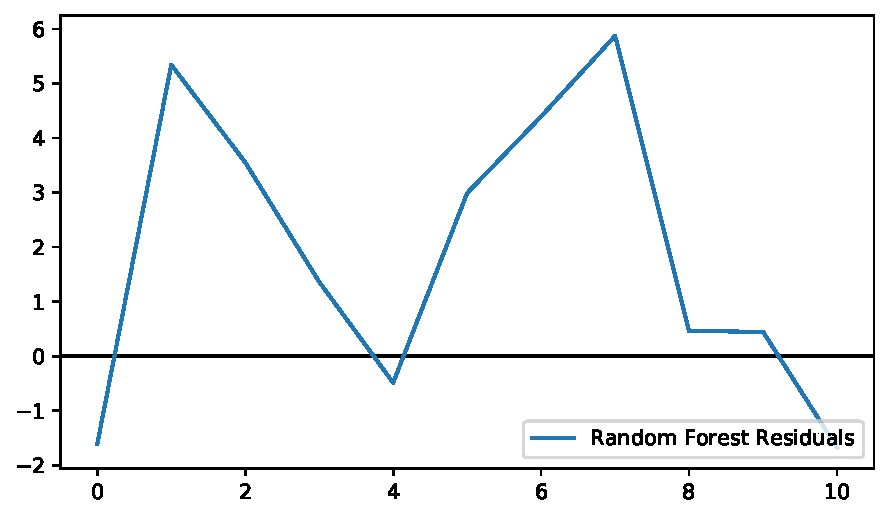
\includegraphics[width=.3\textwidth]{residuals-RandomForest.pdf} 
  \caption{Distribuição dos Erros de cada modelo. Como esperado, todos os erros flutuam em torno da média 0. } 
\end{figure}

\subsection{Regressão Linear Dinâmica com Filtragem Exponencial}

Com o fim de termos uma baseline com a qual compararmos os modelos de Deep
Learning, aplicaremos o modelo proposto em \citep{grecialin}.
Para tal criamos as janelas de dados de treinamento e teste
como explicado anteriormente nesse trabalho. 

Primeiramente apresentamos a variação do erro de treino em
função do parâmetro $t_d$ i.e. o tamanho do conjunto de treino para cada
regressão. Apresentamos os resultados com e sem a aplicação da filtragem
proposta no trabalho \citep{grecialin}.

\begin{figure}[H]
  \centering
  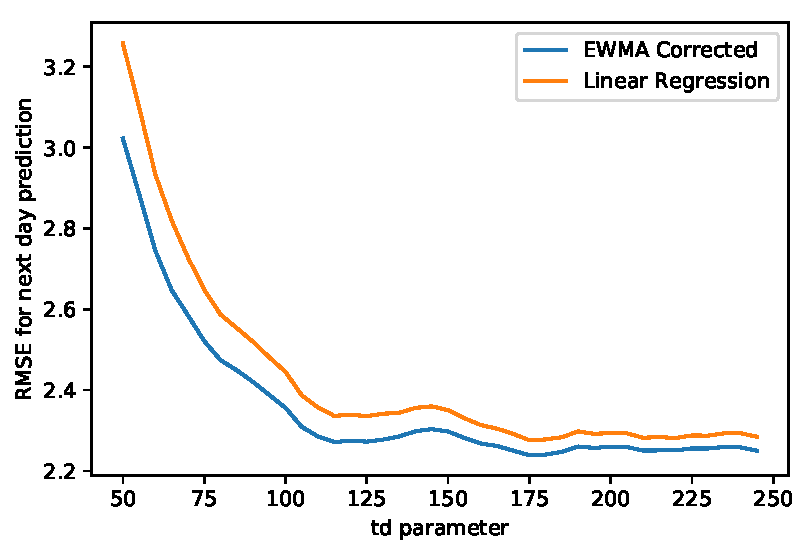
\includegraphics[width=0.9\columnwidth]{tdparameter.pdf}
  \caption{Erro de treino em função do parâmetro $t_d$}
  \label{fig:tdparam}
\end{figure}

Os resultados do modelo em todo o período de validação, bem como o erro são
reportados a seguir:

\begin{figure}[H]
  \centering
  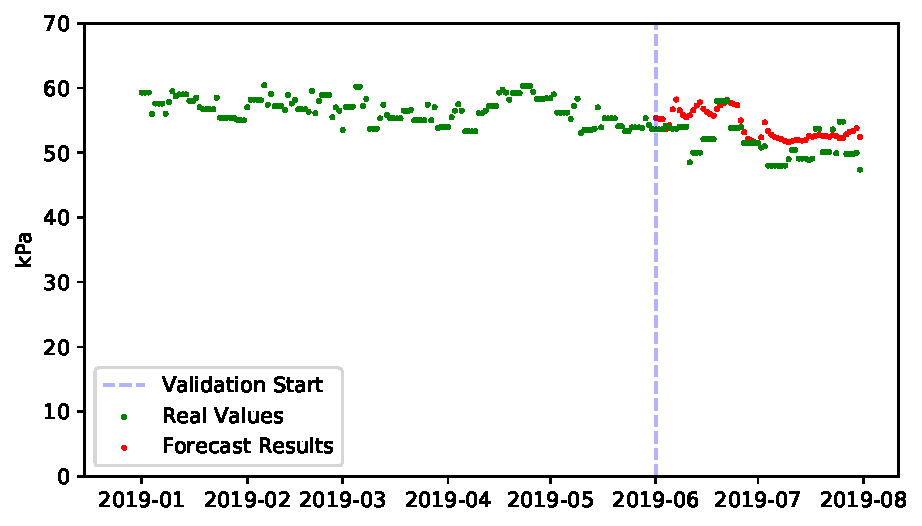
\includegraphics[width=0.9\columnwidth]{forecast_lin_reg_win.pdf}
  \caption{Predições no conjunto de validação do modelo de regressão linear dinâmico}
  \label{fig:tdparam}
\end{figure}

\begin{center}
  \begin{table}[htbp]
    \caption{RMSE values by forecast span}
    \centering
    \begin{tabular}{rr}
      \hline
      Reg. Linear com Filtragem Exponencial & RMSE\\
      \hline
      24h & 1.79 \\ 
      3d & 1.47\\
      7d & 2.36\\
    \end{tabular}

    \label{tb:rmse_exp}
  \end{table}
\end{center}
São reportadas também a distribuição das predições e dos resíduos do modelo exponencial.

\begin{figure}[H]
  \label{fig:distr_exp}
  \centering
  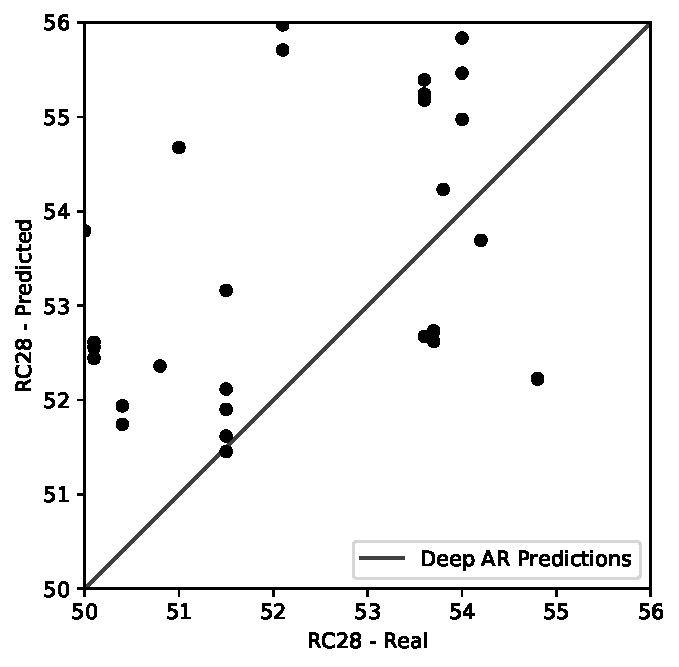
\includegraphics[width=.5\textwidth]{qq_forecast_lin_reg_win.pdf} \hfill
  \caption{Valores reais plotados contra os valores previstos para análise da
    distribuição aprendida pelo modelo exponencial} 
\end{figure}


\begin{figure}[H]
  \label{fig:res_exp}
  \centering
  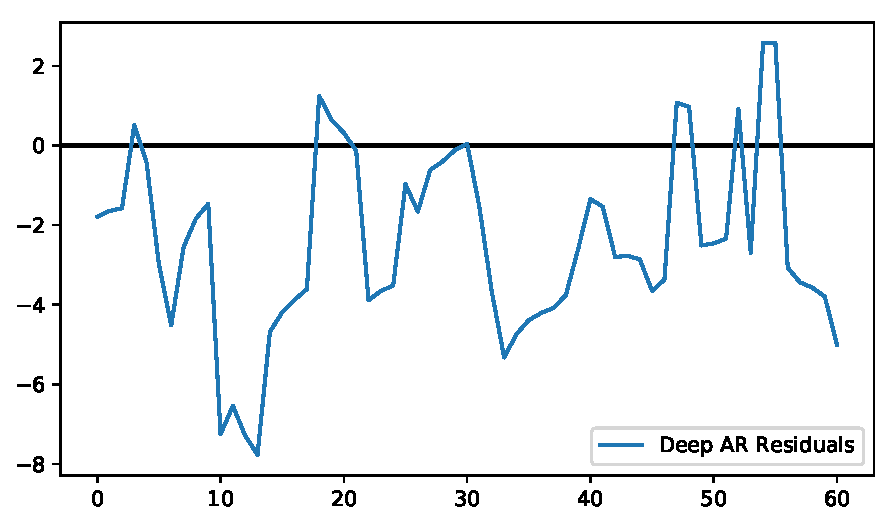
\includegraphics[width=.5\textwidth]{res_forecast_lin_reg_win.pdf} \hfill
  \caption{Distribuição dos resíduos do modelo exponencial} 
\end{figure}

\subsection{Modelos de Aprendizam Profunda Bayesianos para Séries Temporais}


Agora com um tratamento completo do problema como o de previsão de séries
temporais, consideramos os dados sequencialmente, treinando e testando o modelo a partir de janelas de $w$
entradas consumidas em sequência pelo o modelo. A tarefa destes é então gerar
predições que continuem essa janela de dados. Em uma situação real daríamos
alguns dias de dados como entrada e calcularíamos a medida alvo para os próximos dias. 


Como mencionado na introdução desse trabalho, um benefício das técnicas de
Aprendizado Profundo é a de escalar tarefas de aprendizado para datasets de
tamanho muito maior que era possível com modelos clássicos \citep{dlbook}.
Para tarefas de regressão de séries temporais, modelos recentes de Aprendizado
Profundo permitem que sejam usadas diversas séries temporais para a tarefa de
aprendizado. Os modelos poderão então ter parâmetros tanto locais (calculados
para cada série) como globais (dividimos por todas as séries de treinamento).

\subsubsection{Divisão dos dados entre treino e validação}

Com o fim de explorar essa capacidade dos modelos de consumirem diversas séries
temporais, os dados da fábrica de Cajati foram separados por ano e consideramos
cada ano como um exemplo do processo a ser modelado, fornecendo-os separadamente
aos modelos. Os modelos de Aprendizado
Profundo irão então usar parametros locais para cada ano de produção de cimento,
mas globalmente buscar padrões para o funcionamento da fábrica. 

Para cada ano de 2009 até 2019 usaremos os primeiros 11 meses como dados de
treinamento e os últimos 30 dias como dados de validação.



\begin{figure}[H]
  \centering
  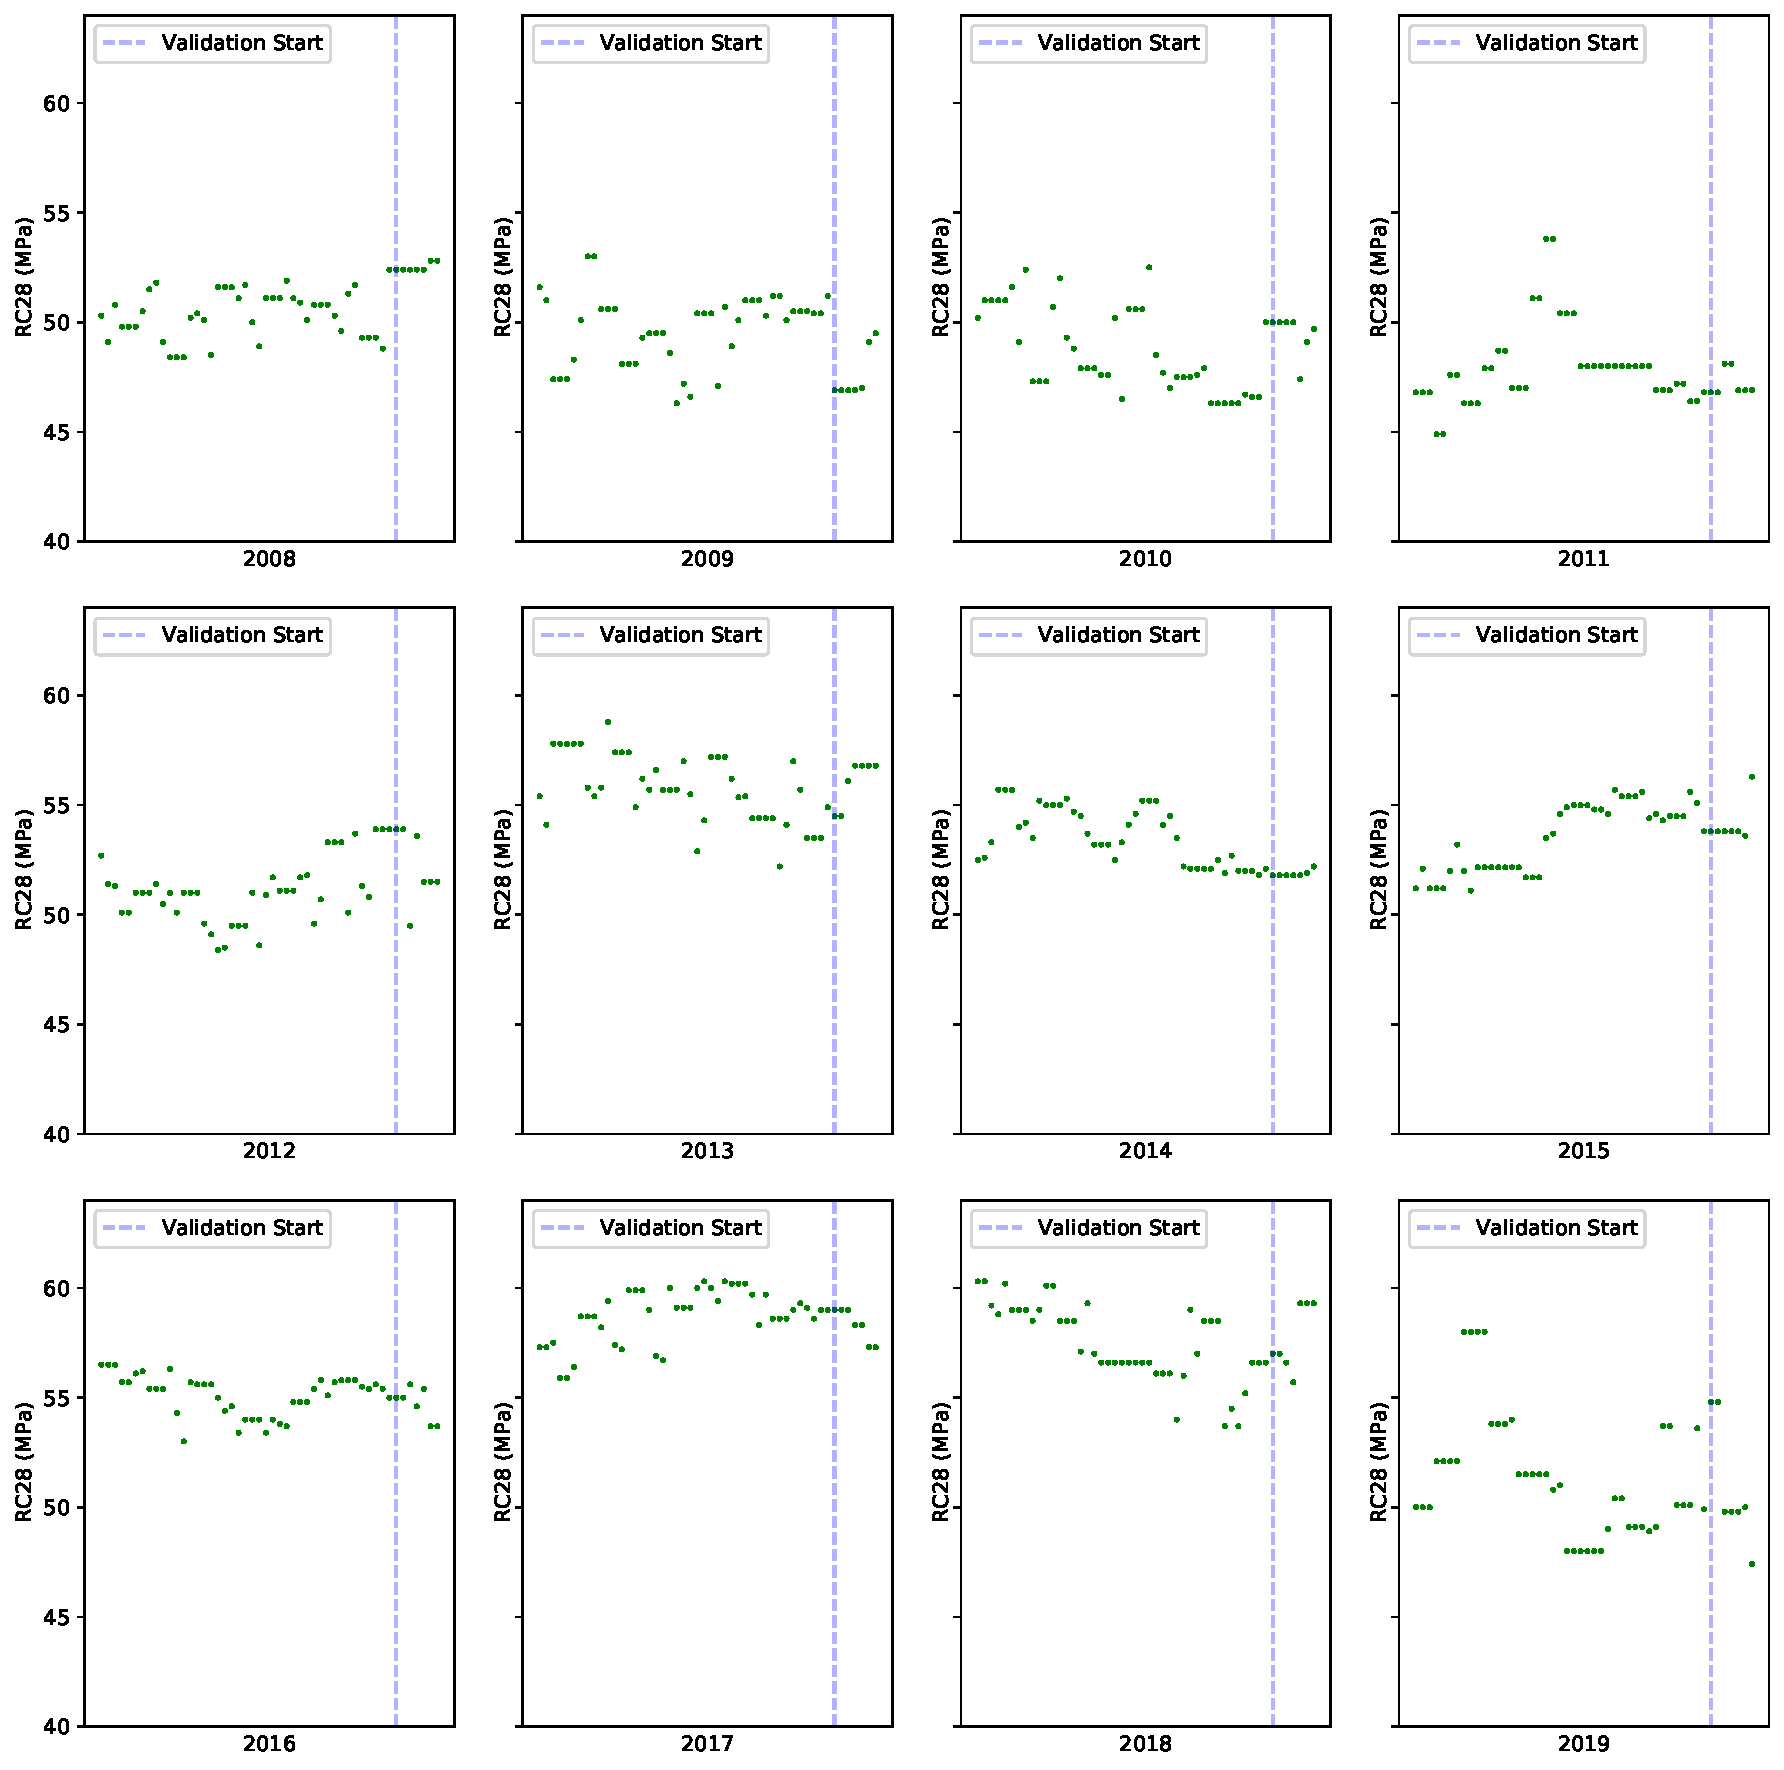
\includegraphics[height=.99\textwidth]{train_val_all_years.pdf} 
  \caption{Os dados são divididos em 11 datasets separados, onde temos por
    dataset 11 meses usados para treino e os últimos dias do ano para validação.} 
  \label{fig:trainvalallyears}
\end{figure}


Usamos a implementacão da biblioteca Pytorch \cite{pytorch} dos modelos, para os Processos Gaussianos usamos a biblioteca GPyTorch \cite{gpytorch}. As tuplas de treino são da forma $(RC28_{t},\{\})$. 

Para os modelos DeepAR e Encoder-Decoder-Forecaster, as predições começam após
uma janela inteira de dias ser codificada pelas redes Encoder.
Apenas então os modelos terão informação para gerar predições. O Modelo Deep
Factors não necessita de uma janela pois sua arquitetura permite e emissão de
predições imediatamente após o primeiro timestep ser recebido,
e o Processo Gaussiano gera incertezas para todo o dataset de validação ao mesmo tempo, visto que é uma operação matricial. \\

Na Tabela~\ref{tb:rmse} reportamos os erros para predições imediatamente no
começo após o fim do último dia de dados usados para treino. Iremos mostrar o
erro para o dia seguinte, três dias depois e então uma semana após o último dia
de dados usados para treinamento.

\begin{center}
\begin{table}[htbp]
\caption{RMSE values by forecast span}
\centering
\begin{tabular}{rr}
\hline
Deep Factors & RMSE\\
\hline
24h & 0.18\\
3d & 2.36\\
7d & 1.83\\
\hline
Deep AR & RMSE\\
\hline
  24h & 0.07\\
3d & 1.37\\
7d & 1.44\\
\hline
Encoder Decoder & RMSE\\
\hline
24h & 0.06\\
3d & 0.44\\
7d & 0.80\\
\end{tabular}

\label{tb:rmse}
\end{table}
\end{center}

A Imagem \ref{fig:distr} compara as distribuições previstas para o mês
de dados de validação pelos 3 modelos:

\begin{figure}[H]
\centering
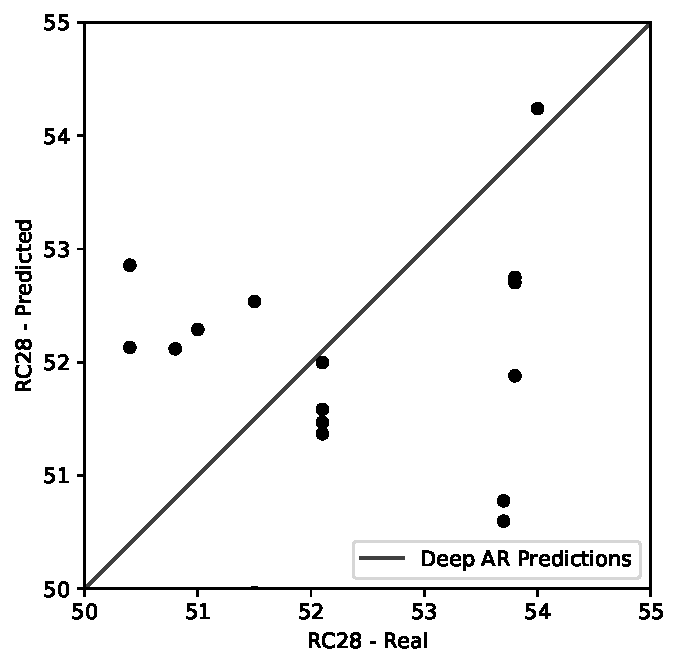
\includegraphics[width=.3\textwidth]{qq_deep_ar.pdf} \hfill
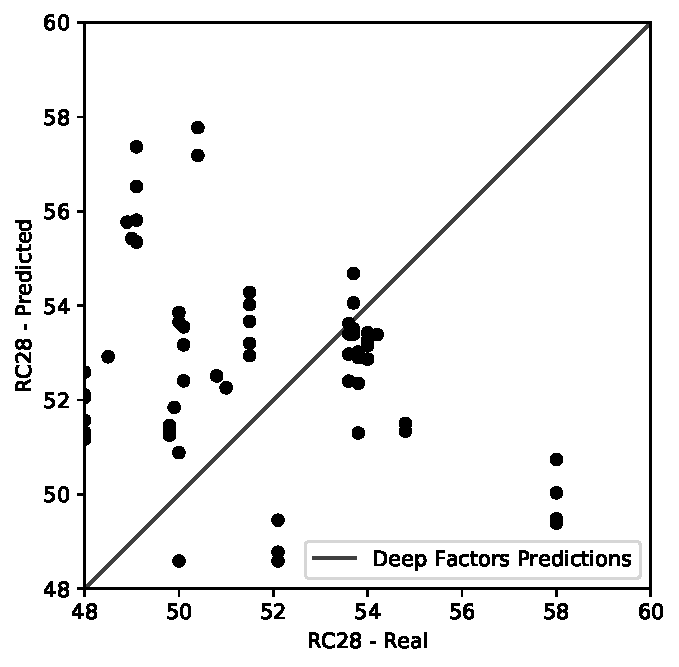
\includegraphics[width=.3\textwidth]{qq_deep_factors.pdf} \hfill
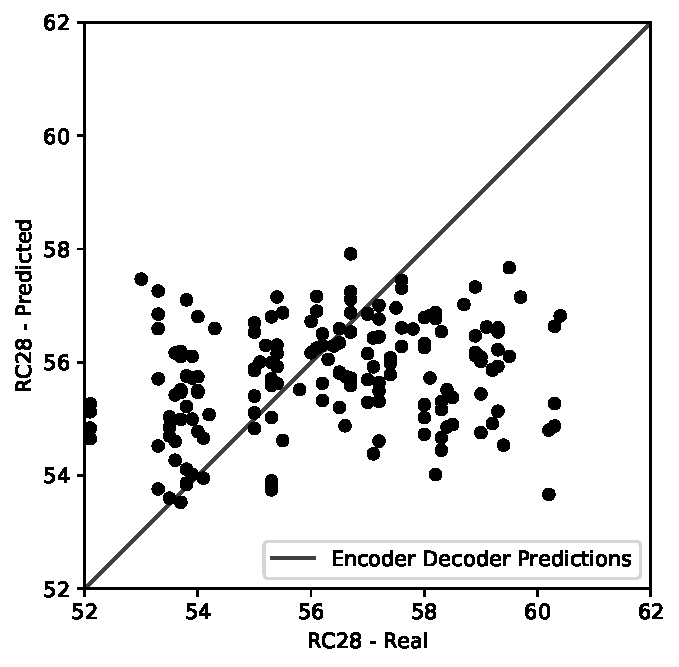
\includegraphics[width=.3\textwidth]{qq_enc_dec.pdf} 
\caption{Valores reais plotados contra os valores previstos para análise da distribuição aprendida por cada modelo} 
\label{fig:distr}
\end{figure}


Finalmente, os valores e incertezas previstos pelos modelos são mostrados nas
Figuras~\ref{fig:fordeepar},\ref{fig:fordeepfactors} e \ref{fig:forencdec}. Nas
figuras são representados as margens de incerteza para $50\%$ e $90\%$ das predições.

\begin{figure}[H]
  \centering
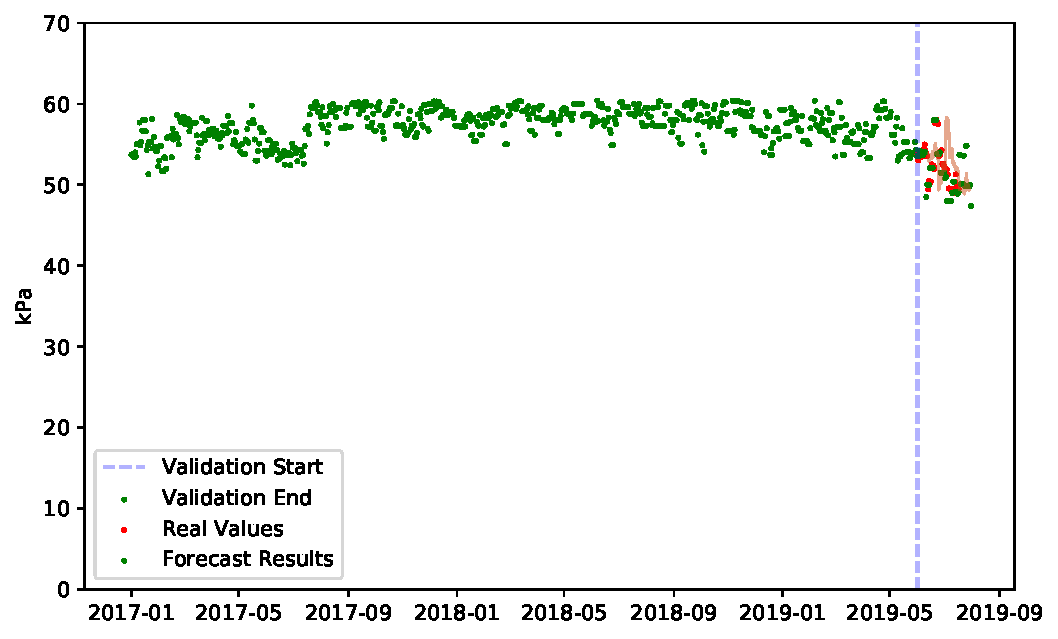
\includegraphics[height=.3\textwidth]{forecast_deep_ar.pdf} 
\caption{Predição para todos os dados de validação para o modelo Deep AR}
\label{fig:fordeepar}
\end{figure}

\begin{figure}[H]
  \centering
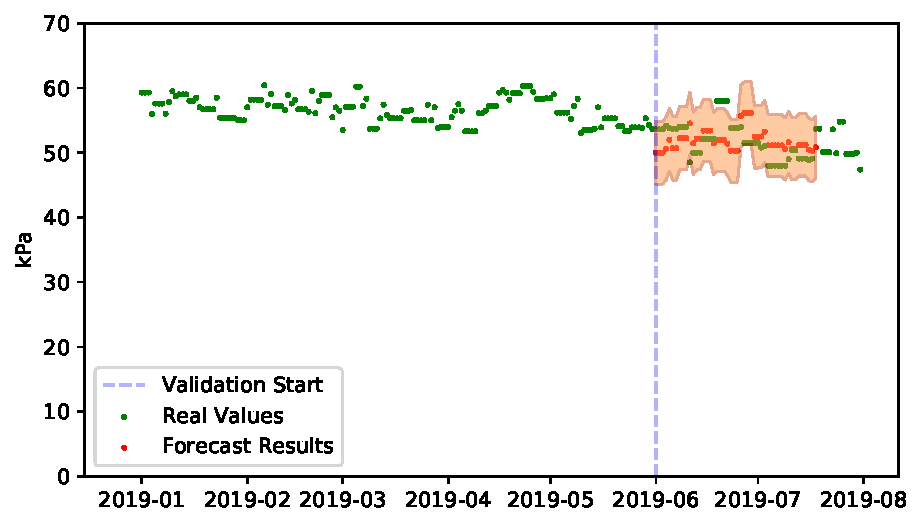
\includegraphics[height=.3\textwidth]{forecast_deep_factors.pdf} 
\caption{Predição para todos os dados de validação para o modelo Deep Factors}
\label{fig:fordeepfactors}
\end{figure}

\begin{figure}[H]
  \centering
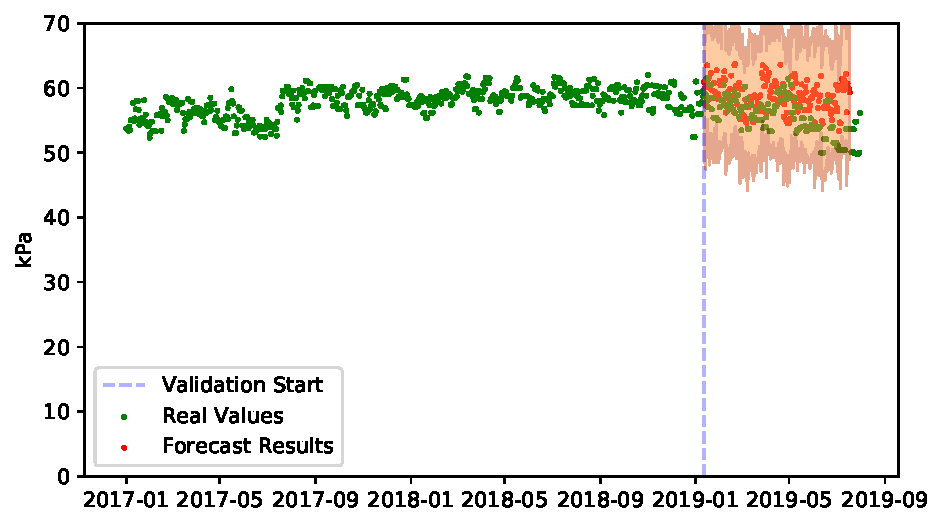
\includegraphics[height=.3\textwidth]{forecast_enc_dec.pdf} 
\caption{Predição para todos os dados de validação para o modelo Encoder Decoder Forecaster} 
\label{fig:forencdec}
\end{figure}


Para modelagem de séries temporais, é também comum estudarmos o resíduo das
predições. Idealmente o resíduo deve ter uma distribuição próxima a uma normal
com média zero, significando que esse erro dos modelos não contém nenhuma parte
não-aleatória que poderia ter sido capturada durante o treino. 

\begin{figure}[H]
\label{fig:res}
\centering
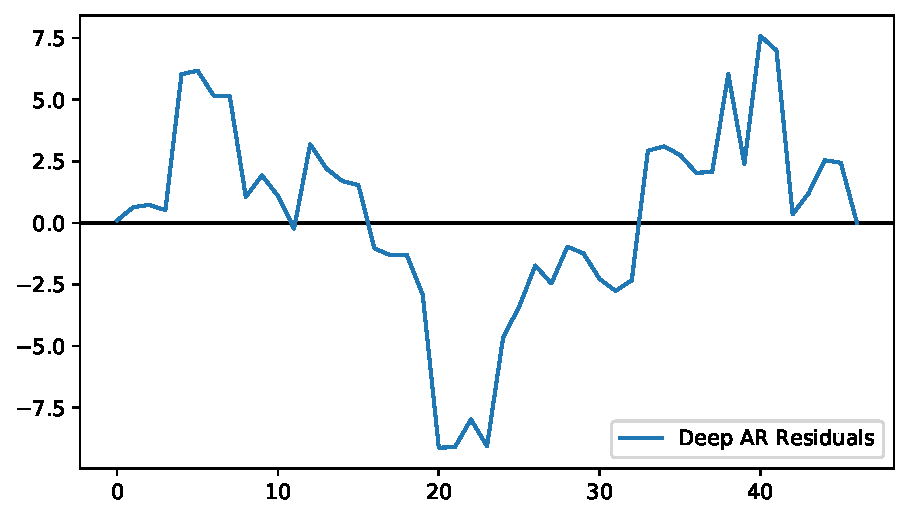
\includegraphics[width=.3\textwidth]{res_deep_ar.pdf} \hfill
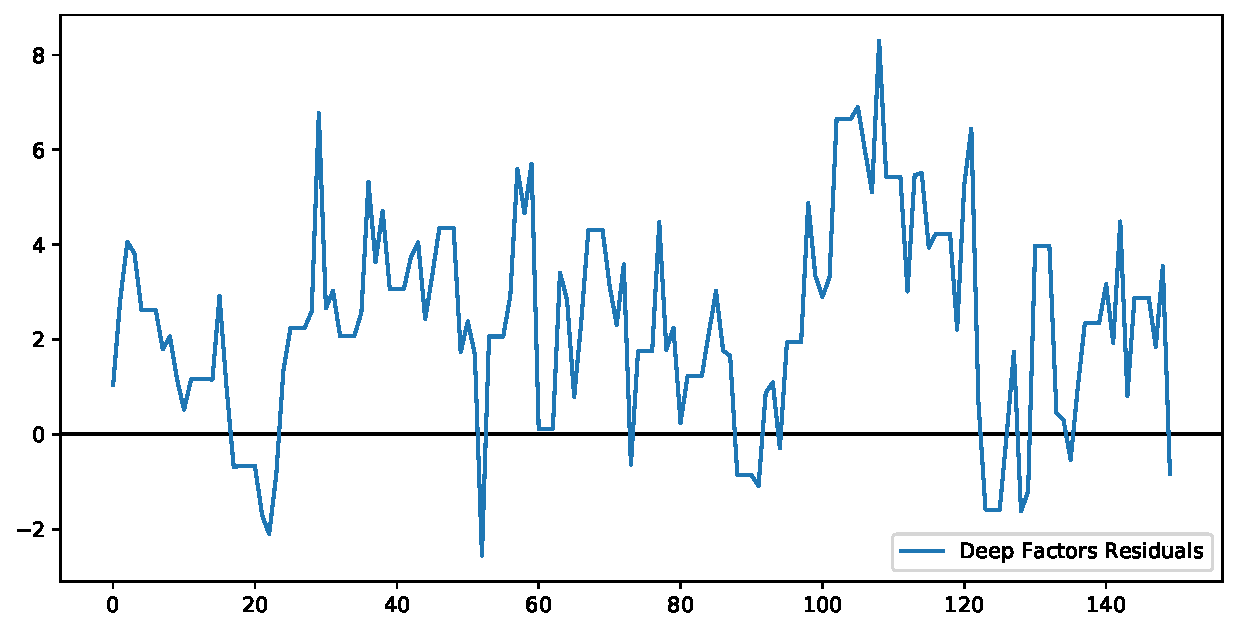
\includegraphics[width=.3\textwidth]{res_deep_factors.pdf} \hfill
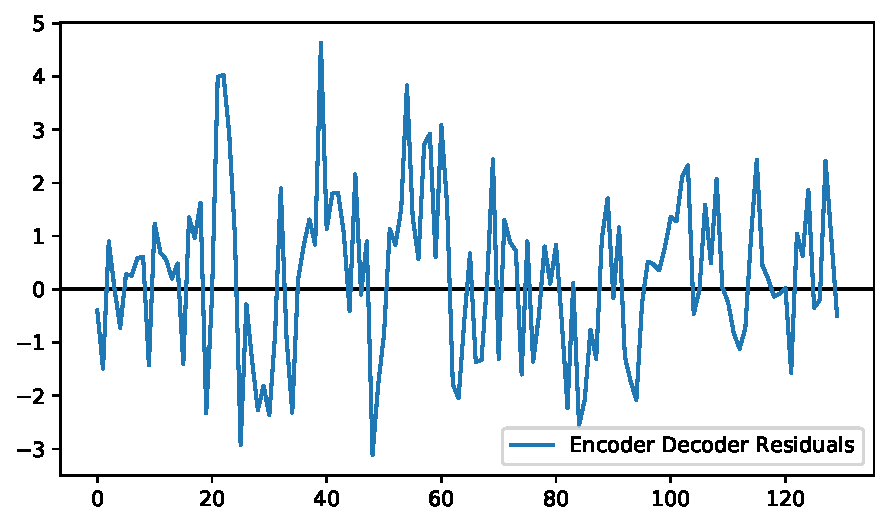
\includegraphics[width=.3\textwidth]{res_enc_dec.pdf} 
\caption{Distribuição dos Erros de cada modelo. Como esperado, todos os erros flutuam em torno da média 0. } 
\end{figure}


Os modelos de DL obtiveram um erro menor na predição do dia seguinte bem como em
horizontes próximos de tempo, tanto em relação aos modelos não-temporais como em
relação ao modelo filtrado exponencialmente.

\begin{center}
  \begin{table}[htbp]
    \caption{Comparação dos modelos de Deep Learning e o modelo Linear}
    \centering
  \begin{tabular}{l|llll}
    \cline{2-4}
    & \multicolumn{1}{l|}{RMSE 24h} & \multicolumn{1}{l|}{RMSE 48h} & \multicolumn{1}{l|}{RMSE 72h} &  \\ \cline{1-4}
    \multicolumn{1}{|l|}{DeepAR}               &               0.07                &          1.37                     &           1.44                    &  \\ \cline{1-1}
    \multicolumn{1}{|l|}{Enc-Dec-Forecaster}   &                   0.06            &        0.44                       &       0.80                        &  \\ \cline{1-1}
    \multicolumn{1}{|l|}{Deep Factors}         &              0.18                 &           2.36                    &                   1.83            &  \\ \cline{1-1}
    \multicolumn{1}{|l|}{Linear Coupled Model} &                  1.79             &       1.47                        &     2.36                          &  \\ \cline{1-1}
  \end{tabular}
  \end{table}
\end{center}
% Local Variables:
% TeX-master: "../quali"
% End:
